\documentclass[11pt]{article}
\usepackage[margin=18mm,headheight=22pt]{geometry}
\usepackage{amsmath}
\usepackage{fontspec}
\usepackage{unicode-math}
\setmainfont{NewCM10}[Extension=.otf,UprightFont=*-Book,BoldFont=*-Bold,ItalicFont=*-BookItalic,BoldItalicFont=*-BoldItalic]
\setsansfont{NewCMSans10}[Extension=.otf,UprightFont=*-Book,BoldFont=*-Bold,ItalicFont=*-BookOblique,BoldItalicFont=*-BoldOblique]
\setmathfont{NewCMMath-Book.otf}
\usepackage{xcolor}
\definecolor{FAUblue}{HTML}{04316A}
\definecolor{Paperblue}{HTML}{EEF2F7}
\definecolor{EEIgold}{HTML}{CC9C42}
\usepackage{etoolbox,enumitem,booktabs,tabularx,array,needspace,microtype}
\usepackage[most]{tcolorbox}
\usepackage{titlesec,fancyhdr}
\usepackage[hidelinks]{hyperref}
\usepackage{draftwatermark}
\SetWatermarkText{Made by Thanate Amornjiraporn (Focus)}
\SetWatermarkColor{black!7}\SetWatermarkFontSize{30pt}\SetWatermarkAngle{45}
\setlength{\parindent}{0pt}
\setlength{\parskip}{5pt}
\setlist{itemsep=2pt,topsep=3pt,leftmargin=1.6em,beginpenalty=10000,endpenalty=10000}
\raggedbottom
\clubpenalty=10000 \widowpenalty=10000 \displaywidowpenalty=10000 \interlinepenalty=10000
\setcounter{secnumdepth}{0}
\setcounter{tocdepth}{1}
\pagestyle{fancy}\fancyhf{}
\fancyhead[L]{\small\sffamily\color{FAUblue} From Fundamentals to AI Apocalypse · EEI · Tutorial 2}
\fancyhead[R]{\small\sffamily Tutorial 2: Worked solutions}
\fancyfoot[C]{\small\thepage}
\titleformat{\section}{\Large\bfseries\sffamily\color{FAUblue}}{}{0pt}{}
\titleformat{\subsection}{\large\bfseries\sffamily\color{FAUblue}}{}{0pt}{}
\titlespacing*{\section}{0pt}{16pt}{6pt}
\preto\section{\Needspace{8\baselineskip}}
\preto\subsection{\Needspace{6\baselineskip}}
\newtcolorbox{equationcard}[1]{colback=Paperblue,colframe=Paperblue,boxrule=0pt,arc=0pt,left=10pt,right=10pt,top=6pt,bottom=6pt,title={#1},fonttitle=\small\bfseries\sffamily,coltitle=FAUblue,before skip=8pt,after skip=8pt}
\newtcolorbox{workedbox}[1]{colback=white,colframe=EEIgold,boxrule=0pt,leftrule=3pt,arc=0pt,left=10pt,top=4pt,bottom=4pt,title={#1},fonttitle=\small\bfseries\sffamily,coltitle=FAUblue,attach title to upper={\par},before skip=8pt,after skip=8pt}
\newtcolorbox{recallbox}[1]{colback=white,colframe=FAUblue,boxrule=0pt,leftrule=3pt,arc=0pt,left=10pt,top=4pt,bottom=4pt,title={#1},fonttitle=\small\bfseries\sffamily,coltitle=FAUblue,attach title to upper={\par},before skip=8pt,after skip=8pt}
\usepackage{environ}
\newsavebox\measurebox
% Typeset the section once invisibly to measure it; start a new page if it will not fit in what is left.
\makeatletter
\newif\ifkeep@measuring
\NewEnviron{keepsection}{%
  \ifkeep@measuring \BODY \else
    \edef\keep@sec{\the\value{section}}\edef\keep@sub{\the\value{subsection}}%
    \setbox\measurebox\vbox{\hsize\linewidth\keep@measuringtrue\def\Needspace##1{}\BODY}%
    \setcounter{section}{\keep@sec}\setcounter{subsection}{\keep@sub}%
    \dimen2=\ht\measurebox \advance\dimen2\dp\measurebox
    \dimen@=\textheight
    \ifdim\pagegoal<\maxdimen
      \dimen@=\pagegoal \advance\dimen@-\pagetotal
      \ifdim\dimen2>\dimen@ \clearpage \dimen@=\textheight \fi
    \fi
    % if it fits, nothing inside may force an early break
    \ifdim\dimen2>\dimen@ \BODY \else \begingroup\def\Needspace##1{}\BODY\endgroup \fi
  \fi}
\makeatother
\newtcolorbox{notebox}{colback=Paperblue,colframe=Paperblue,boxrule=0pt,arc=0pt,left=8pt,right=8pt,top=4pt,bottom=4pt,before skip=6pt,after skip=6pt}
\newtcolorbox{plainbox}{colback=white,colframe=FAUblue,boxrule=0pt,leftrule=3pt,arc=0pt,left=10pt,right=8pt,top=4pt,bottom=4pt,before skip=6pt,after skip=8pt}
\usetikzlibrary{arrows.meta}
\title{\sffamily\bfseries\color{FAUblue}Tutorial 2: Worked solutions}
\author{Electrical Engineering I \ensuremath{\cdot} Module 92315 \ensuremath{\cdot} Tutorial 2\\[2pt]\small From Fundamentals to AI Apocalypse · personal study guide}
\date{}
\begin{document}
\maketitle
\begingroup\footnotesize\setlength{\parskip}{0pt}\tableofcontents\endgroup
\clearpage

\Needspace{8\baselineskip}
{\large These solutions build total charge by integrating the volume charge density over the region where it exists. Track the coordinate-dependent volume element and the density’s support.}


\begin{keepsection}
\Needspace{9\baselineskip}
\section{Task 4: Cylinder coordinates}

\Needspace{6\baselineskip}
The space charge density is constant, ϱ\textsubscript{V} = ϱ\textsubscript{0}, in the hollow cylindrical region a \ensuremath{\leq} \textit{ρ} \ensuremath{\leq} b, 0 \ensuremath{\leq} \textit{φ} \ensuremath{\leq} 2π, 0 \ensuremath{\leq} \textit{z} \ensuremath{\leq} c, and zero outside. Assume 0 \ensuremath{\leq} a \ensuremath{<} b and c \ensuremath{>} 0.

\Needspace{9\baselineskip}
\textbf{Connected topic:} Charge densities (§1.6): the total charge is the volume integral of the density. The cylindrical volume element is in Appendix A.5.

\Needspace{14\baselineskip}
\begin{center}
\begin{minipage}[t]{0.950\linewidth}\centering
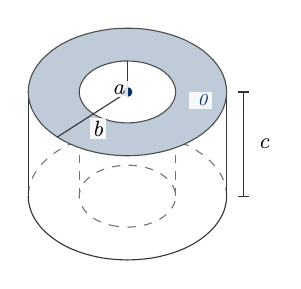
\begin{tikzpicture}[line join=round]
\draw[black!55,dashed] plot[smooth,tension=0.5] coordinates {(2.628,-2.241) (2.623,-2.171) (2.608,-2.101) (2.585,-2.032) (2.552,-1.964) (2.509,-1.899) (2.459,-1.836) (2.399,-1.777) (2.333,-1.721) (2.259,-1.669) (2.178,-1.620) (2.092,-1.577) (1.998,-1.539) (1.901,-1.507) (1.798,-1.480) (1.694,-1.458) (1.588,-1.444) (1.478,-1.435) (1.368,-1.431) (1.258,-1.435) (1.148,-1.444) (1.042,-1.458) (0.938,-1.480) (0.835,-1.507) (0.738,-1.539) (0.644,-1.577) (0.558,-1.620) (0.477,-1.669) (0.403,-1.721) (0.337,-1.777) (0.277,-1.836) (0.227,-1.899) (0.184,-1.964) (0.151,-2.032) (0.128,-2.101) (0.113,-2.171) (0.108,-2.241)};
\draw[black!80] plot[smooth,tension=0.5] coordinates {(0.108,-2.241) (0.113,-2.311) (0.128,-2.381) (0.151,-2.450) (0.184,-2.518) (0.227,-2.583) (0.277,-2.646) (0.337,-2.705) (0.403,-2.761) (0.477,-2.813) (0.558,-2.862) (0.644,-2.905) (0.738,-2.943) (0.835,-2.975) (0.938,-3.002) (1.042,-3.024) (1.148,-3.038) (1.258,-3.047) (1.368,-3.051) (1.478,-3.047) (1.588,-3.038) (1.694,-3.024) (1.798,-3.002) (1.901,-2.975) (1.998,-2.943) (2.092,-2.905) (2.178,-2.862) (2.259,-2.813) (2.333,-2.761) (2.399,-2.705) (2.459,-2.646) (2.509,-2.583) (2.552,-2.518) (2.585,-2.450) (2.608,-2.381) (2.623,-2.311) (2.628,-2.241)};
\draw[black!80] (2.628,-2.241) -- (2.628,-0.918);
\draw[black!80] (0.108,-2.241) -- (0.108,-0.918);
\draw[black!55,dashed] (1.980,-2.241) -- (1.980,-0.918);
\draw[black!55,dashed] (0.756,-2.241) -- (0.756,-0.918);
\draw[black!55,dashed] plot[smooth,tension=0.5] coordinates {(1.159,-2.610) (1.235,-2.624) (1.314,-2.633) (1.395,-2.633) (1.474,-2.628) (1.552,-2.615) (1.627,-2.597) (1.697,-2.572) (1.762,-2.542) (1.820,-2.507) (1.870,-2.466) (1.912,-2.423) (1.942,-2.376) (1.966,-2.326) (1.978,-2.275) (1.980,-2.223) (1.971,-2.173) (1.951,-2.122) (1.922,-2.075) (1.885,-2.030) (1.836,-1.989) (1.782,-1.951) (1.719,-1.919) (1.651,-1.892) (1.577,-1.872) (1.501,-1.858) (1.422,-1.849) (1.341,-1.849) (1.262,-1.854) (1.184,-1.867) (1.109,-1.885) (1.039,-1.910) (0.974,-1.940) (0.916,-1.975) (0.866,-2.016) (0.824,-2.059) (0.794,-2.106) (0.770,-2.156) (0.758,-2.207) (0.756,-2.259) (0.765,-2.309) (0.785,-2.360) (0.814,-2.407) (0.851,-2.452) (0.900,-2.493) (0.954,-2.531) (1.017,-2.563) (1.085,-2.590) (1.159,-2.610)};
\filldraw[draw=black!70,fill=FAUblue!25] (0.938,-1.678) -- (1.042,-1.699) -- (1.148,-1.715) -- (1.258,-1.724) -- (1.368,-1.728) -- (1.478,-1.724) -- (1.588,-1.715) -- (1.694,-1.699) -- (1.798,-1.678) -- (1.901,-1.651) -- (1.998,-1.618) -- (2.092,-1.580) -- (2.178,-1.537) -- (2.259,-1.490) -- (2.333,-1.438) -- (2.399,-1.382) -- (2.459,-1.323) -- (2.509,-1.260) -- (2.552,-1.193) -- (2.585,-1.127) -- (2.608,-1.058) -- (2.623,-0.988) -- (2.628,-0.918) -- (2.623,-0.846) -- (2.608,-0.776) -- (2.585,-0.707) -- (2.552,-0.641) -- (2.509,-0.574) -- (2.459,-0.513) -- (2.399,-0.454) -- (2.333,-0.396) -- (2.259,-0.344) -- (2.178,-0.297) -- (2.092,-0.254) -- (1.998,-0.216) -- (1.901,-0.184) -- (1.798,-0.157) -- (1.694,-0.135) -- (1.588,-0.119) -- (1.478,-0.110) -- (1.368,-0.108) -- (1.258,-0.110) -- (1.148,-0.119) -- (1.042,-0.135) -- (0.938,-0.157) -- (0.835,-0.184) -- (0.738,-0.216) -- (0.644,-0.254) -- (0.558,-0.297) -- (0.477,-0.344) -- (0.403,-0.396) -- (0.337,-0.454) -- (0.277,-0.513) -- (0.227,-0.574) -- (0.184,-0.641) -- (0.151,-0.707) -- (0.128,-0.776) -- (0.113,-0.846) -- (0.108,-0.918) -- (0.113,-0.988) -- (0.128,-1.058) -- (0.151,-1.127) -- (0.184,-1.193) -- (0.227,-1.260) -- (0.277,-1.323) -- (0.337,-1.382) -- (0.403,-1.438) -- (0.477,-1.490) -- (0.558,-1.537) -- (0.644,-1.580) -- (0.738,-1.618) -- (0.835,-1.651) -- (0.938,-1.678) -- cycle;
\filldraw[draw=black!70,fill=white] (1.159,-1.287) -- (1.235,-1.301) -- (1.314,-1.309) -- (1.395,-1.310) -- (1.474,-1.305) -- (1.552,-1.292) -- (1.627,-1.274) -- (1.697,-1.249) -- (1.762,-1.219) -- (1.820,-1.183) -- (1.870,-1.143) -- (1.912,-1.100) -- (1.942,-1.051) -- (1.966,-1.003) -- (1.978,-0.952) -- (1.980,-0.900) -- (1.971,-0.850) -- (1.951,-0.799) -- (1.922,-0.751) -- (1.885,-0.706) -- (1.836,-0.664) -- (1.782,-0.626) -- (1.719,-0.596) -- (1.651,-0.569) -- (1.577,-0.547) -- (1.501,-0.533) -- (1.422,-0.526) -- (1.341,-0.524) -- (1.262,-0.529) -- (1.184,-0.542) -- (1.109,-0.562) -- (1.039,-0.585) -- (0.974,-0.616) -- (0.916,-0.652) -- (0.866,-0.691) -- (0.824,-0.736) -- (0.794,-0.783) -- (0.770,-0.832) -- (0.758,-0.884) -- (0.756,-0.934) -- (0.765,-0.986) -- (0.785,-1.035) -- (0.814,-1.084) -- (0.851,-1.129) -- (0.900,-1.170) -- (0.954,-1.208) -- (1.017,-1.240) -- (1.085,-1.265) -- (1.159,-1.287) -- cycle;
\draw[black!80] (1.368,-0.918) -- (1.368,-0.524);
\draw[black!80] (1.368,-0.918) -- (0.477,-1.490);
\fill[FAUblue] (1.368,-0.918) circle (0.063);
\node[fill=white,fill opacity=0.85,text opacity=1,inner sep=1pt,font=\footnotesize] at (1.260,-0.883) {\textit{a}};
\node[fill=white,fill opacity=0.85,text opacity=1,inner sep=1pt,font=\footnotesize] at (0.994,-1.384) {\textit{b}};
\draw[black!80] (2.844,-2.241) -- (2.844,-0.918);
\draw[black!80] (2.772,-2.241) -- (2.916,-2.241);
\draw[black!80] (2.772,-0.918) -- (2.916,-0.918);
\node[anchor=west,fill=white,fill opacity=0.85,text opacity=1,inner sep=1pt,font=\footnotesize] at (2.988,-1.579) {\textit{c}};
\node[text=FAUblue,fill=white,fill opacity=0.85,text opacity=1,inner sep=1pt,font=\footnotesize] at (2.290,-1.022) {\textit{ϱ\textsubscript{0}}};
\end{tikzpicture}\par\smallskip{\small\raggedright \textbf{Only the wall is charged.} The density ϱ\textsubscript{0} fills the region between the radii \textit{a} and \textit{b} (shaded on top) over the height \textit{c}; the bore inside radius \textit{a} is empty, so the radial integral starts at \textit{a}.\par}\end{minipage}
\end{center}

\begin{keepsection}
\Needspace{7\baselineskip}
\subsection{4: Total charge in the hollow cylinder}

\Needspace{4\baselineskip}
Try first: write the cylindrical volume element, then integrate across the inner and outer radii, the full angle, and the height.

\nopagebreak[4]{\small\itshape Answers: see “Task 4: Cylinder coordinates” under Answers at the end.}
\end{keepsection}
\end{keepsection}

\begin{keepsection}
\Needspace{9\baselineskip}
\section{Task 5: Spherical coordinates}

\Needspace{6\baselineskip}
The density varies radially as ϱ\textsubscript{V}(r) = ϱ\textsubscript{0}r\textsuperscript{2}/a\textsuperscript{2} inside a sphere of radius a and is zero for r \ensuremath{>} a. Assume a \ensuremath{>} 0.

\Needspace{9\baselineskip}
\textbf{Connected topic:} Charge densities (§1.6): each thin spherical shell contributes its density times its volume. The spherical volume element is in Appendix A.5.

\Needspace{14\baselineskip}
\begin{center}
\begin{minipage}[t]{0.950\linewidth}\centering
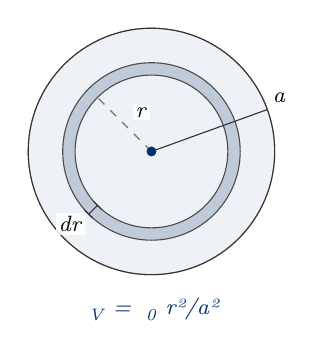
\begin{tikzpicture}[line join=round]
\filldraw[draw=black!40,fill=Paperblue,even odd rule] (2.232,-2.232) circle (1.565) ;
\filldraw[draw=black!70,fill=FAUblue!25,even odd rule] (2.232,-2.232) circle (1.127) (2.232,-2.232) circle (0.970);
\draw[black!80] (2.232,-2.232) circle (1.565);
\draw[black!80] (2.232,-2.232) -- (3.703,-1.700);
\node[anchor=west,fill=white,fill opacity=0.85,text opacity=1,inner sep=1pt,font=\footnotesize] at (3.731,-1.553) {\textit{a}};
\draw[black!55,dashed] (2.232,-2.232) -- (1.546,-1.546);
\node[anchor=west,fill=white,fill opacity=0.85,text opacity=1,inner sep=1pt,font=\footnotesize] at (1.990,-1.738) {\textit{r}};
\draw[black!80] (1.546,-2.918) -- (1.435,-3.029);
\draw[black!80] (1.597,-2.968) -- (1.496,-2.867);
\draw[black!80] (1.486,-3.080) -- (1.384,-2.978);
\node[anchor=east,fill=white,fill opacity=0.85,text opacity=1,inner sep=1pt,font=\footnotesize] at (1.401,-3.153) {\textit{dr}};
\fill[FAUblue] (2.232,-2.232) circle (0.063);
\node[text=FAUblue,fill=white,fill opacity=0.85,text opacity=1,inner sep=1pt,font=\footnotesize] at (2.232,-4.235) {\textit{ϱ\textsubscript{V} = ϱ\textsubscript{0} r²/a²}};
\end{tikzpicture}\par\smallskip{\small\raggedright \textbf{Add up thin shells.} The shell at radius \textit{r} and thickness d\textit{r} (shaded) has volume 4π\textit{r}\textsuperscript{2} d\textit{r} and density ϱ\textsubscript{0}\textit{r}\textsuperscript{2}/\textit{a}\textsuperscript{2}; the outer shells are both larger and denser.\par}\end{minipage}
\end{center}

\begin{keepsection}
\Needspace{7\baselineskip}
\subsection{5: Total charge in the sphere}

\Needspace{4\baselineskip}
Try first: multiply the radial density by the spherical shell volume 4πr²dr and integrate from the centre to a.

\nopagebreak[4]{\small\itshape Answers: see “Task 5: Spherical coordinates” under Answers at the end.}
\end{keepsection}
\end{keepsection}


\clearpage
\section{Answers}
\begin{keepsection}\subsection{Task 4: Cylinder coordinates}

\begin{workedbox}{4 \ensuremath{\cdot} Cylindrical volume integral}
\Needspace{10\baselineskip}
\begin{enumerate}
\item \Needspace{5\baselineskip}
Total charge is the volume integral of volume charge density over the charged region. In cylindrical coordinates, a small volume is a wedge-shaped piece with volume ρ dρ dφ dz:

\begin{equation*}{Q}\, =\, \iiint_{{V}} \, ϱ_{\mathrm{V}}\, \mathrm{d}{V},\quad \, \quad \, \mathrm{d}{V}\, =\, ρ\, \mathrm{d}ρ\, \mathrm{d}φ\, \mathrm{d}{z}\end{equation*}
\item \Needspace{5\baselineskip}
Substitute the constant density and the stated limits. The inner radius a excludes the empty central cylinder:

\Needspace{4\baselineskip}
\begin{equation*}{Q}\, =\, ϱ_{0}\, \int_{0}^{{c}} \, \int_{0}^{2π} \, \int_{{a}}^{{b}} \, ρ\, \mathrm{d}ρ\, \mathrm{d}φ\, \mathrm{d}{z}\end{equation*}

\begin{equation*}{Q}\, =\, ϱ_{0}\, \int_{0}^{{c}} \, \int_{0}^{2π} \, \left[\dfrac{ρ^{2}}{2}\right]_{{a}}^{{b}}\, \mathrm{d}φ\, \mathrm{d}{z}\end{equation*}
\item \Needspace{4\baselineskip}
Evaluate the radial term, then the full revolution and cylinder height:

\Needspace{4\baselineskip}
\begin{equation*}{Q}\, =\, ϱ_{0}\, \dfrac{{b}^{2}\, -\, {a}^{2}}{2}\, (2π)\, {c}\end{equation*}

\Needspace{5\baselineskip}
\begin{equation*}{Q}\, =\, ϱ_{0}\, π({b}^{2}\, -\, {a}^{2}){c}\end{equation*}

The sign follows the sign of ϱ\textsubscript{0}. \textbf{Check:} the factor π(b² \ensuremath{-} a²)c is exactly the hollow cylinder’s volume, and ϱ\textsubscript{0} times volume has units C.
\end{enumerate}
\end{workedbox}

\end{keepsection}
\begin{keepsection}\subsection{Task 5: Spherical coordinates}

\begin{workedbox}{5 \ensuremath{\cdot} Spherical volume integral}
\Needspace{8\baselineskip}
\begin{enumerate}
\item \Needspace{5\baselineskip}
For a spherically symmetric density, integrate over concentric shells. A shell at radius r has volume 4πr²dr, and only radii 0 through a contain charge:

\begin{equation*}{Q}\, =\, \iiint_{{V}} \, ϱ_{\mathrm{V}}\, \mathrm{d}{V}\, =\, 4π\, \int_{0}^{{a}} \, ϱ_{\mathrm{V}}({r})\, {r}^{2}\, \mathrm{d}{r}\end{equation*}
\item \Needspace{4\baselineskip}
Insert the given density. One factor r² comes from the shell area and another from ϱ\textsubscript{V}:

\Needspace{4\baselineskip}
\begin{equation*}{Q}\, =\, 4π\, \int_{0}^{{a}} \, ϱ_{0}\, \dfrac{{r}^{2}}{{a}^{2}}\, {r}^{2}\, \mathrm{d}{r}\end{equation*}

\begin{equation*}{Q}\, =\, \dfrac{4πϱ_{0}}{{a}^{2}}\, \int_{0}^{{a}} \, {r}^{4}\, \mathrm{d}{r}\end{equation*}
\item \Needspace{4\baselineskip}
Integrate \textit{r}\textsuperscript{4} and apply both limits:

\Needspace{4\baselineskip}
\begin{equation*}{Q}\, =\, \dfrac{4πϱ_{0}}{{a}^{2}}\, \left[\dfrac{{r}^{5}}{5}\right]_{0}^{{a}}\end{equation*}

\Needspace{5\baselineskip}
\begin{equation*}{Q}\, =\, \dfrac{4πϱ_{0}\, {a}^{3}}{5}\end{equation*}

The sign follows ϱ\textsubscript{0}. \textbf{Check:} the average density is 3ϱ\textsubscript{0}/5, giving (3ϱ\textsubscript{0}/5)(4πa³/3), the same result.
\end{enumerate}
\end{workedbox}

\end{keepsection}

\vfill{\small Personal worked-solution guide based on the supplied EE1 Tutorial Task sheet, written in my own words; no tutorial text or figures are reproduced. Not an official FAU publication; check course details against current material. Made by \textbf{Thanate Amornjiraporn (Focus)}.}

\end{document}
